\documentclass[]{article}
\usepackage{lmodern}
\usepackage{amssymb,amsmath}
\usepackage{ifxetex,ifluatex}
\usepackage{fixltx2e} % provides \textsubscript
\ifnum 0\ifxetex 1\fi\ifluatex 1\fi=0 % if pdftex
  \usepackage[T1]{fontenc}
  \usepackage[utf8]{inputenc}
\else % if luatex or xelatex
  \ifxetex
    \usepackage{mathspec}
  \else
    \usepackage{fontspec}
  \fi
  \defaultfontfeatures{Ligatures=TeX,Scale=MatchLowercase}
\fi
% use upquote if available, for straight quotes in verbatim environments
\IfFileExists{upquote.sty}{\usepackage{upquote}}{}
% use microtype if available
\IfFileExists{microtype.sty}{%
\usepackage{microtype}
\UseMicrotypeSet[protrusion]{basicmath} % disable protrusion for tt fonts
}{}
\usepackage[margin=1in]{geometry}
\usepackage{hyperref}
\hypersetup{unicode=true,
            pdfborder={0 0 0},
            breaklinks=true}
\urlstyle{same}  % don't use monospace font for urls
\usepackage{color}
\usepackage{fancyvrb}
\newcommand{\VerbBar}{|}
\newcommand{\VERB}{\Verb[commandchars=\\\{\}]}
\DefineVerbatimEnvironment{Highlighting}{Verbatim}{commandchars=\\\{\}}
% Add ',fontsize=\small' for more characters per line
\usepackage{framed}
\definecolor{shadecolor}{RGB}{248,248,248}
\newenvironment{Shaded}{\begin{snugshade}}{\end{snugshade}}
\newcommand{\KeywordTok}[1]{\textcolor[rgb]{0.13,0.29,0.53}{\textbf{#1}}}
\newcommand{\DataTypeTok}[1]{\textcolor[rgb]{0.13,0.29,0.53}{#1}}
\newcommand{\DecValTok}[1]{\textcolor[rgb]{0.00,0.00,0.81}{#1}}
\newcommand{\BaseNTok}[1]{\textcolor[rgb]{0.00,0.00,0.81}{#1}}
\newcommand{\FloatTok}[1]{\textcolor[rgb]{0.00,0.00,0.81}{#1}}
\newcommand{\ConstantTok}[1]{\textcolor[rgb]{0.00,0.00,0.00}{#1}}
\newcommand{\CharTok}[1]{\textcolor[rgb]{0.31,0.60,0.02}{#1}}
\newcommand{\SpecialCharTok}[1]{\textcolor[rgb]{0.00,0.00,0.00}{#1}}
\newcommand{\StringTok}[1]{\textcolor[rgb]{0.31,0.60,0.02}{#1}}
\newcommand{\VerbatimStringTok}[1]{\textcolor[rgb]{0.31,0.60,0.02}{#1}}
\newcommand{\SpecialStringTok}[1]{\textcolor[rgb]{0.31,0.60,0.02}{#1}}
\newcommand{\ImportTok}[1]{#1}
\newcommand{\CommentTok}[1]{\textcolor[rgb]{0.56,0.35,0.01}{\textit{#1}}}
\newcommand{\DocumentationTok}[1]{\textcolor[rgb]{0.56,0.35,0.01}{\textbf{\textit{#1}}}}
\newcommand{\AnnotationTok}[1]{\textcolor[rgb]{0.56,0.35,0.01}{\textbf{\textit{#1}}}}
\newcommand{\CommentVarTok}[1]{\textcolor[rgb]{0.56,0.35,0.01}{\textbf{\textit{#1}}}}
\newcommand{\OtherTok}[1]{\textcolor[rgb]{0.56,0.35,0.01}{#1}}
\newcommand{\FunctionTok}[1]{\textcolor[rgb]{0.00,0.00,0.00}{#1}}
\newcommand{\VariableTok}[1]{\textcolor[rgb]{0.00,0.00,0.00}{#1}}
\newcommand{\ControlFlowTok}[1]{\textcolor[rgb]{0.13,0.29,0.53}{\textbf{#1}}}
\newcommand{\OperatorTok}[1]{\textcolor[rgb]{0.81,0.36,0.00}{\textbf{#1}}}
\newcommand{\BuiltInTok}[1]{#1}
\newcommand{\ExtensionTok}[1]{#1}
\newcommand{\PreprocessorTok}[1]{\textcolor[rgb]{0.56,0.35,0.01}{\textit{#1}}}
\newcommand{\AttributeTok}[1]{\textcolor[rgb]{0.77,0.63,0.00}{#1}}
\newcommand{\RegionMarkerTok}[1]{#1}
\newcommand{\InformationTok}[1]{\textcolor[rgb]{0.56,0.35,0.01}{\textbf{\textit{#1}}}}
\newcommand{\WarningTok}[1]{\textcolor[rgb]{0.56,0.35,0.01}{\textbf{\textit{#1}}}}
\newcommand{\AlertTok}[1]{\textcolor[rgb]{0.94,0.16,0.16}{#1}}
\newcommand{\ErrorTok}[1]{\textcolor[rgb]{0.64,0.00,0.00}{\textbf{#1}}}
\newcommand{\NormalTok}[1]{#1}
\usepackage{graphicx,grffile}
\makeatletter
\def\maxwidth{\ifdim\Gin@nat@width>\linewidth\linewidth\else\Gin@nat@width\fi}
\def\maxheight{\ifdim\Gin@nat@height>\textheight\textheight\else\Gin@nat@height\fi}
\makeatother
% Scale images if necessary, so that they will not overflow the page
% margins by default, and it is still possible to overwrite the defaults
% using explicit options in \includegraphics[width, height, ...]{}
\setkeys{Gin}{width=\maxwidth,height=\maxheight,keepaspectratio}
\IfFileExists{parskip.sty}{%
\usepackage{parskip}
}{% else
\setlength{\parindent}{0pt}
\setlength{\parskip}{6pt plus 2pt minus 1pt}
}
\setlength{\emergencystretch}{3em}  % prevent overfull lines
\providecommand{\tightlist}{%
  \setlength{\itemsep}{0pt}\setlength{\parskip}{0pt}}
\setcounter{secnumdepth}{0}
% Redefines (sub)paragraphs to behave more like sections
\ifx\paragraph\undefined\else
\let\oldparagraph\paragraph
\renewcommand{\paragraph}[1]{\oldparagraph{#1}\mbox{}}
\fi
\ifx\subparagraph\undefined\else
\let\oldsubparagraph\subparagraph
\renewcommand{\subparagraph}[1]{\oldsubparagraph{#1}\mbox{}}
\fi

%%% Use protect on footnotes to avoid problems with footnotes in titles
\let\rmarkdownfootnote\footnote%
\def\footnote{\protect\rmarkdownfootnote}

%%% Change title format to be more compact
\usepackage{titling}

% Create subtitle command for use in maketitle
\newcommand{\subtitle}[1]{
  \posttitle{
    \begin{center}\large#1\end{center}
    }
}

\setlength{\droptitle}{-2em}

  \title{}
    \pretitle{\vspace{\droptitle}}
  \posttitle{}
    \author{}
    \preauthor{}\postauthor{}
    \date{}
    \predate{}\postdate{}
  

\begin{document}

\begin{Shaded}
\begin{Highlighting}[]
\NormalTok{knitr}\OperatorTok{::}\NormalTok{opts_chunk}\OperatorTok{$}\KeywordTok{set}\NormalTok{(}\DataTypeTok{echo =} \OtherTok{TRUE}\NormalTok{)}
\NormalTok{nsims <-}\StringTok{ }\DecValTok{100000} \CommentTok{#set number of simulations}
\KeywordTok{require}\NormalTok{(mvtnorm, }\DataTypeTok{quietly =} \OtherTok{TRUE}\NormalTok{)}
\KeywordTok{require}\NormalTok{(MASS, }\DataTypeTok{quietly =} \OtherTok{TRUE}\NormalTok{)}
\KeywordTok{require}\NormalTok{(afex, }\DataTypeTok{quietly =} \OtherTok{TRUE}\NormalTok{)}
\KeywordTok{require}\NormalTok{(emmeans, }\DataTypeTok{quietly =} \OtherTok{TRUE}\NormalTok{)}
\KeywordTok{require}\NormalTok{(ggplot2, }\DataTypeTok{quietly =} \OtherTok{TRUE}\NormalTok{)}
\KeywordTok{require}\NormalTok{(gridExtra, }\DataTypeTok{quietly =} \OtherTok{TRUE}\NormalTok{)}
\KeywordTok{require}\NormalTok{(reshape2, }\DataTypeTok{quietly =} \OtherTok{TRUE}\NormalTok{)}
\KeywordTok{require}\NormalTok{(pwr, }\DataTypeTok{quietly =} \OtherTok{TRUE}\NormalTok{)}
\end{Highlighting}
\end{Shaded}

\subsection{Validation of Power in Mixed
ANOVA}\label{validation-of-power-in-mixed-anova}

We install the functions:

\begin{Shaded}
\begin{Highlighting}[]
\CommentTok{# Install the two functions from GitHub by running the code below:}

\KeywordTok{source}\NormalTok{(}\StringTok{"https://raw.githubusercontent.com/Lakens/ANOVA_power_simulation/master/ANOVA_design.R"}\NormalTok{)}
\KeywordTok{source}\NormalTok{(}\StringTok{"https://raw.githubusercontent.com/Lakens/ANOVA_power_simulation/master/ANOVA_power.R"}\NormalTok{)}
\end{Highlighting}
\end{Shaded}

\subsection{Two by two ANOVA, within-between
design}\label{two-by-two-anova-within-between-design}

We can simulate a Two-Way ANOVA with a specific alpha, sample size and
effect size, to achieve a specified statistical power. We wil try to
reproduce the power analysis by g*power for an F-test, ANOVA: Repeated
measures, within-between interaction.

\begin{figure}
\centering
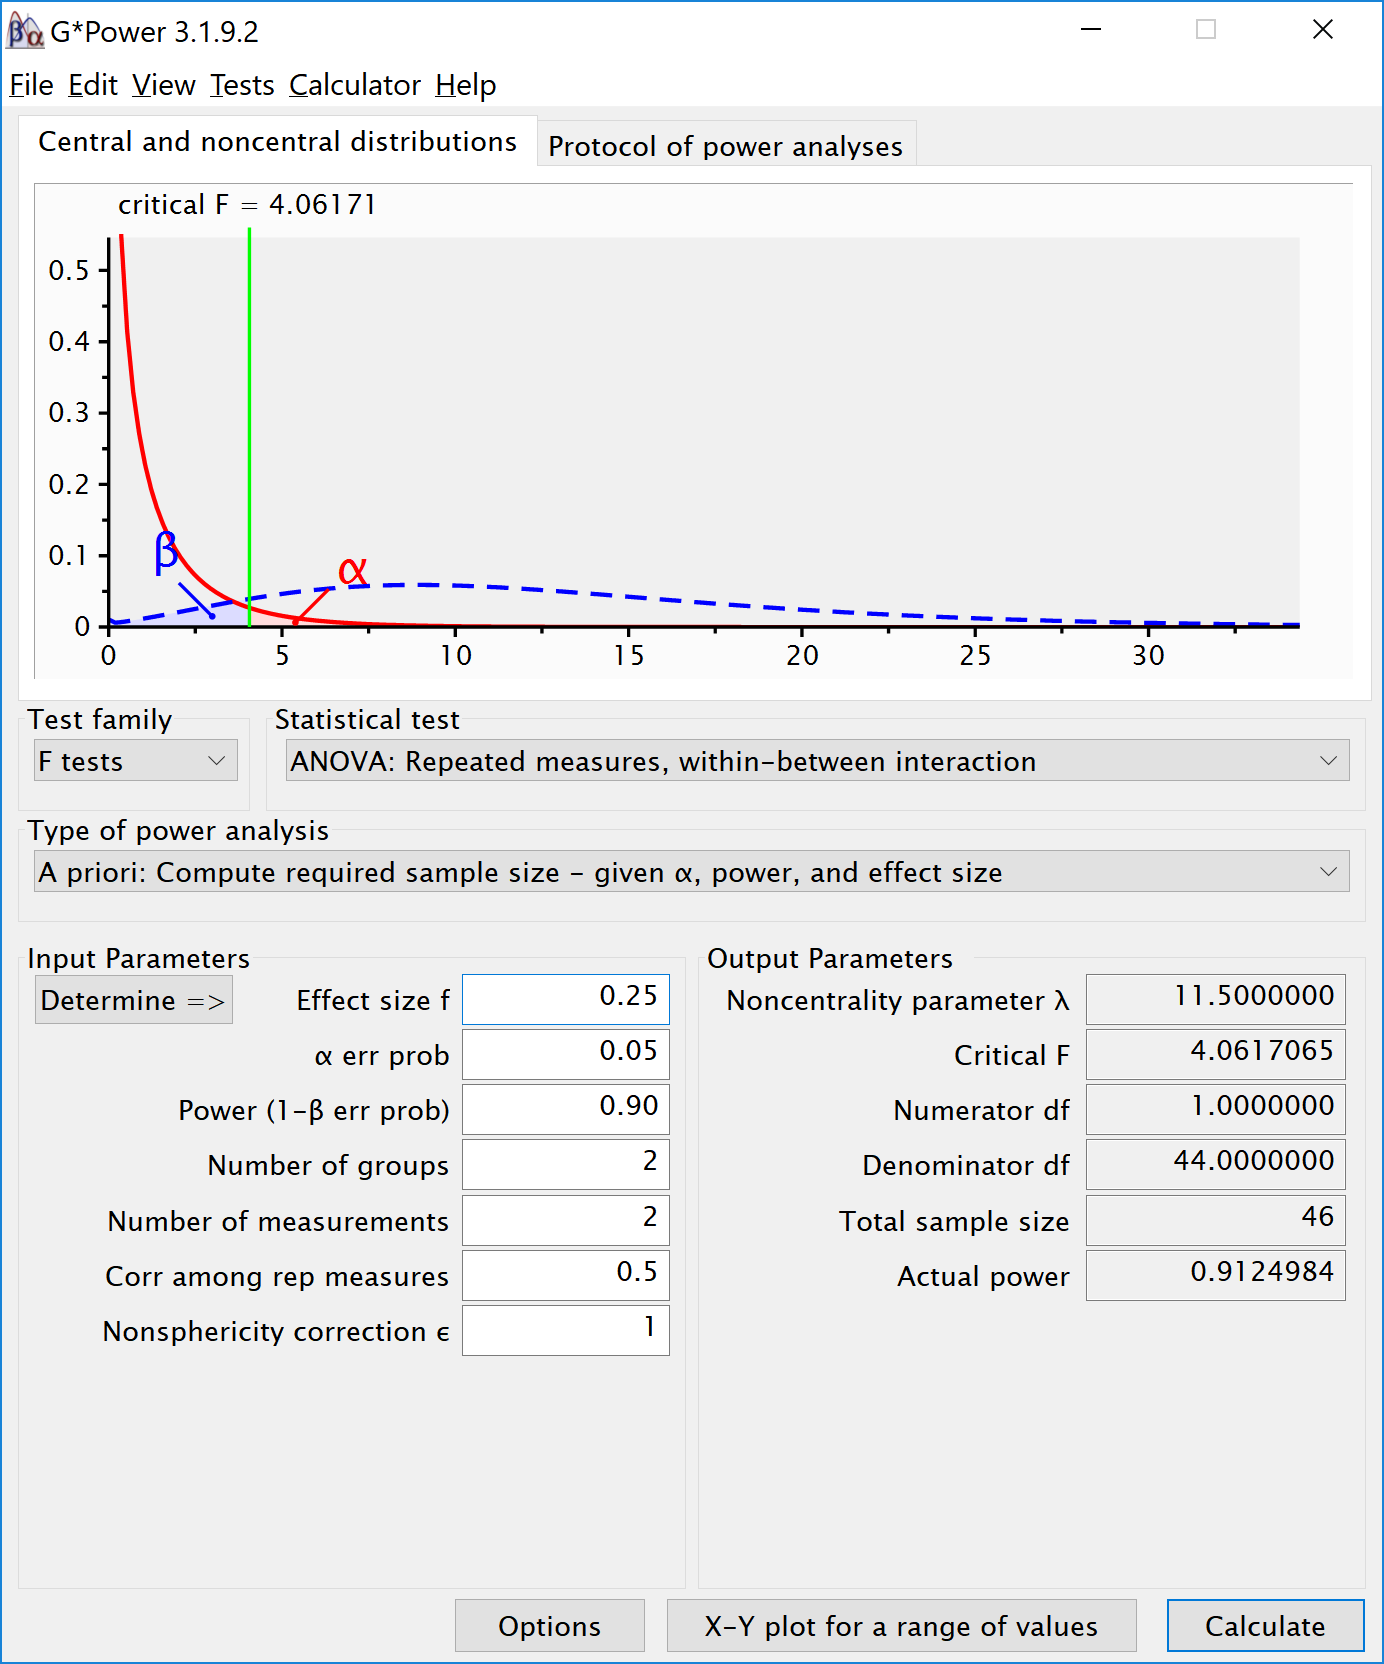
\includegraphics{screenshots/gpower_5.png}
\caption{}
\end{figure}

For the 2-way interaction, the result should be a power of 91.25\% is we
have a total samplesize of 46. Since we have 2 groups in the between
factor that means the sample size per group is 2 (and both these groups
collect 2 repeated measures).

\begin{Shaded}
\begin{Highlighting}[]
\NormalTok{mu <-}\StringTok{ }\KeywordTok{c}\NormalTok{(}\OperatorTok{-}\FloatTok{0.25}\NormalTok{, }\FloatTok{0.25}\NormalTok{, }\FloatTok{0.25}\NormalTok{, }\FloatTok{-0.25}\NormalTok{)}
\NormalTok{n <-}\StringTok{ }\DecValTok{23}
\NormalTok{sd <-}\StringTok{ }\DecValTok{1}
\NormalTok{r <-}\StringTok{ }\FloatTok{0.5}
\NormalTok{string =}\StringTok{ "2w*2b"}
\NormalTok{alpha_level <-}\StringTok{ }\FloatTok{0.05}
\NormalTok{labelnames =}\StringTok{ }\KeywordTok{c}\NormalTok{(}\StringTok{"age"}\NormalTok{, }\StringTok{"old"}\NormalTok{, }\StringTok{"young"}\NormalTok{, }\StringTok{"color"}\NormalTok{, }\StringTok{"blue"}\NormalTok{, }\StringTok{"red"}\NormalTok{)}
\NormalTok{design_result <-}\StringTok{ }\KeywordTok{ANOVA_design}\NormalTok{(}\DataTypeTok{string =}\NormalTok{ string,}
                              \DataTypeTok{n =}\NormalTok{ n, }
                              \DataTypeTok{mu =}\NormalTok{ mu, }
                              \DataTypeTok{sd =}\NormalTok{ sd, }
                              \DataTypeTok{r =}\NormalTok{ r, }
                              \DataTypeTok{labelnames =}\NormalTok{ labelnames)}
\end{Highlighting}
\end{Shaded}

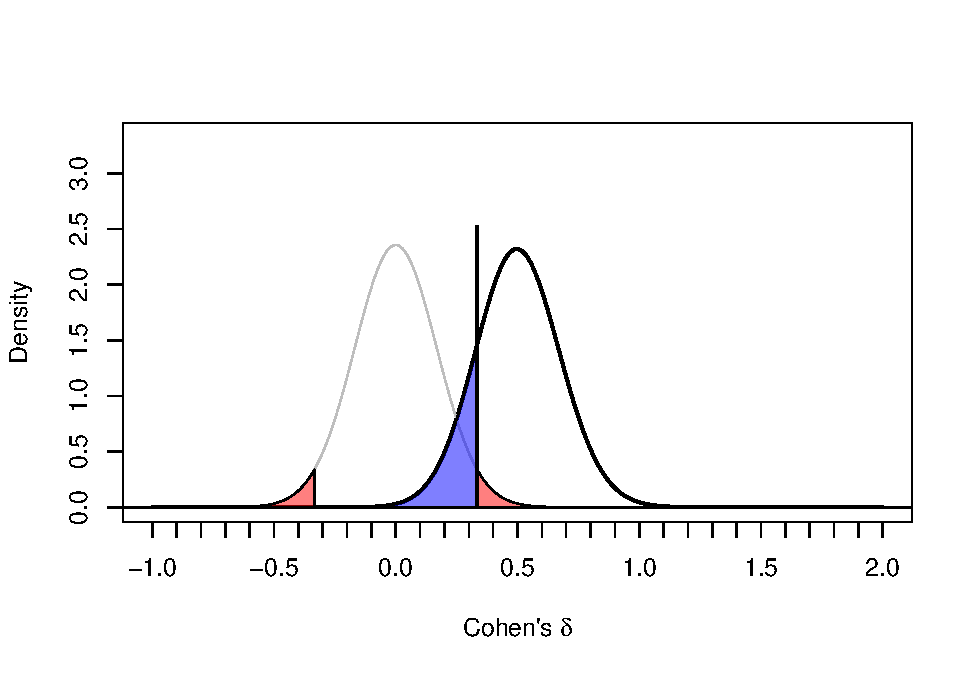
\includegraphics{3.1_validation_power_between_within_2x2_files/figure-latex/unnamed-chunk-2-1.pdf}

\begin{Shaded}
\begin{Highlighting}[]
\NormalTok{simulation_result <-}\StringTok{ }\KeywordTok{ANOVA_power}\NormalTok{(design_result, }\DataTypeTok{alpha =} \FloatTok{0.05}\NormalTok{, }\DataTypeTok{nsims =}\NormalTok{ nsims)}
\end{Highlighting}
\end{Shaded}

\begin{verbatim}
## Power and Effect sizes for ANOVA tests
##                  power effect size
## anova_color      5.087      0.0103
## anova_age        5.105      0.0105
## anova_color:age 91.190      0.2086
## 
## Power and Effect sizes for contrasts
##                                             power effect size
## p_age_old_color_blue_age_old_color_red     38.039      0.5083
## p_age_old_color_blue_age_young_color_blue  62.954      0.5174
## p_age_old_color_blue_age_young_color_red    4.998     -0.0004
## p_age_old_color_red_age_young_color_blue    5.025     -0.0003
## p_age_old_color_red_age_young_color_red    63.078     -0.5178
## p_age_young_color_blue_age_young_color_red 38.033     -0.5085
\end{verbatim}

\subsection{Two by two ANOVA, within-between design Variation
1}\label{two-by-two-anova-within-between-design-variation-1}

We can simulate the same Two-Way ANOVA increasing the correlation to
0.7.

\begin{figure}
\centering
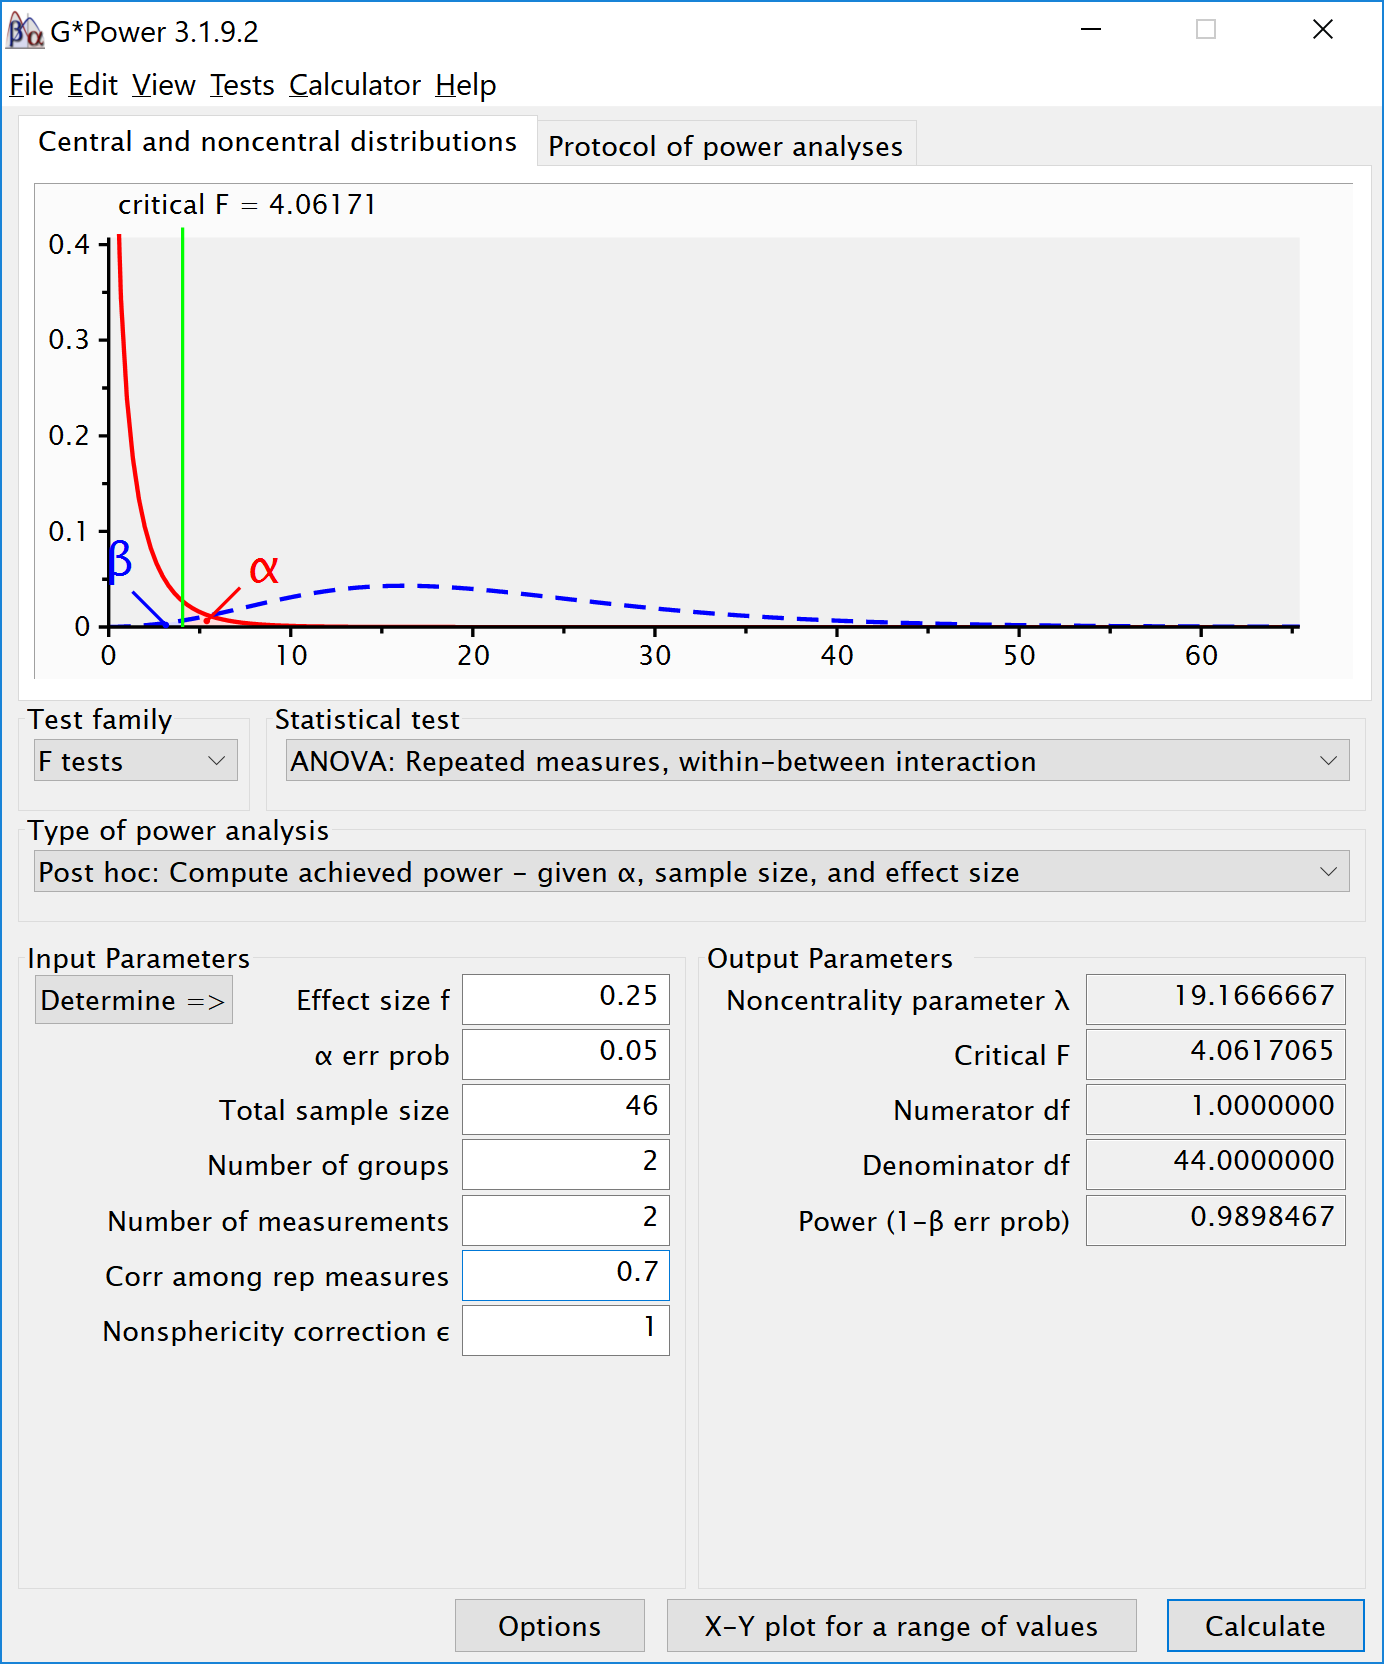
\includegraphics{screenshots/gpower_6.png}
\caption{}
\end{figure}

\begin{Shaded}
\begin{Highlighting}[]
\NormalTok{mu <-}\StringTok{ }\KeywordTok{c}\NormalTok{(}\OperatorTok{-}\FloatTok{0.25}\NormalTok{, }\FloatTok{0.25}\NormalTok{, }\FloatTok{0.25}\NormalTok{, }\FloatTok{-0.25}\NormalTok{)}
\NormalTok{n <-}\StringTok{ }\DecValTok{23}
\NormalTok{sd <-}\StringTok{ }\DecValTok{1}
\NormalTok{r <-}\StringTok{ }\FloatTok{0.7}
\NormalTok{string =}\StringTok{ "2w*2b"}
\NormalTok{alpha_level <-}\StringTok{ }\FloatTok{0.05}
\NormalTok{labelnames =}\StringTok{ }\KeywordTok{c}\NormalTok{(}\StringTok{"age"}\NormalTok{, }\StringTok{"old"}\NormalTok{, }\StringTok{"young"}\NormalTok{, }\StringTok{"color"}\NormalTok{, }\StringTok{"blue"}\NormalTok{, }\StringTok{"red"}\NormalTok{)}
\NormalTok{design_result <-}\StringTok{ }\KeywordTok{ANOVA_design}\NormalTok{(}\DataTypeTok{string =}\NormalTok{ string,}
                              \DataTypeTok{n =}\NormalTok{ n, }
                              \DataTypeTok{mu =}\NormalTok{ mu, }
                              \DataTypeTok{sd =}\NormalTok{ sd, }
                              \DataTypeTok{r =}\NormalTok{ r, }
                              \DataTypeTok{labelnames =}\NormalTok{ labelnames)}
\end{Highlighting}
\end{Shaded}

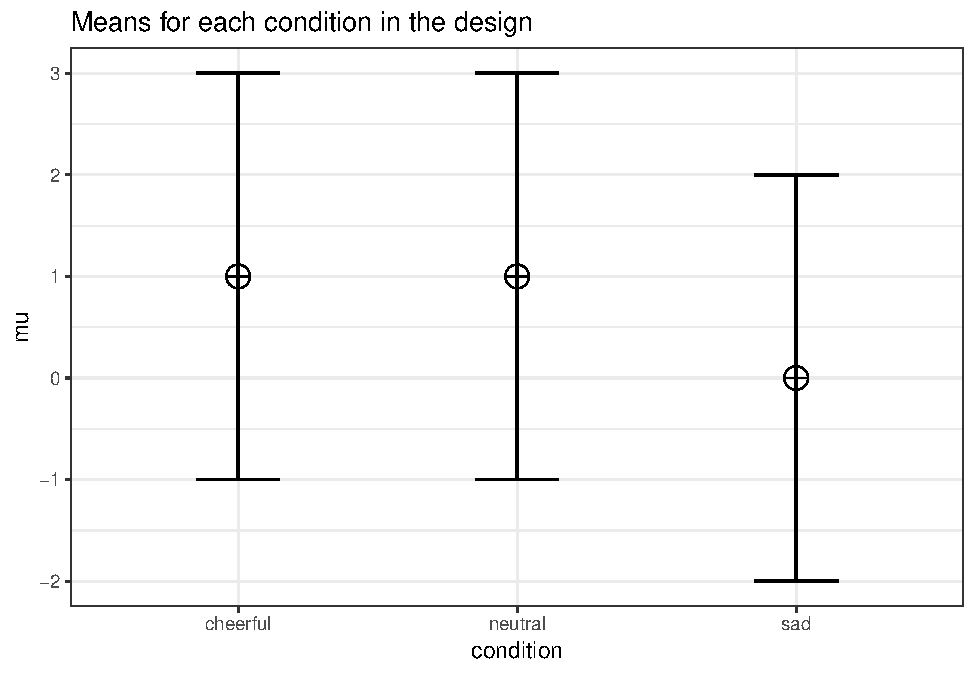
\includegraphics{3.1_validation_power_between_within_2x2_files/figure-latex/unnamed-chunk-3-1.pdf}

\begin{Shaded}
\begin{Highlighting}[]
\NormalTok{simulation_result <-}\StringTok{ }\KeywordTok{ANOVA_power}\NormalTok{(design_result, }\DataTypeTok{alpha =} \FloatTok{0.05}\NormalTok{, }\DataTypeTok{nsims =}\NormalTok{ nsims)}
\end{Highlighting}
\end{Shaded}

\begin{verbatim}
## Power and Effect sizes for ANOVA tests
##                  power effect size
## anova_color      5.025      0.0104
## anova_age        5.120      0.0105
## anova_color:age 98.936      0.3063
## 
## Power and Effect sizes for contrasts
##                                             power effect size
## p_age_old_color_blue_age_old_color_red     38.362      0.5086
## p_age_old_color_blue_age_young_color_blue  83.908      0.6677
## p_age_old_color_blue_age_young_color_red    4.991     -0.0004
## p_age_old_color_red_age_young_color_blue    5.001     -0.0002
## p_age_old_color_red_age_young_color_red    84.022     -0.6692
## p_age_young_color_blue_age_young_color_red 38.155     -0.5085
\end{verbatim}


\end{document}
